\chapter{Introdução}


Segundo a \textit{wikipedia}:
\textit{"Robotics is the branch of technology that deals with the design, construction,
operation, and application of robots,as well as computer systems for their control,
sensory feedback, and information processing"}. As influencias da robótica já
são visíveis na indústria moderna. Ela tem viabilizado o desenvolvimento de peças
precisas, assim como um controle maior do processo. O uso de robôs confere aos
processos industriais precisão e repetibilidade maior que as adquiridas caso
fosse empregado um humano. Isso, além de reduzir o custo de retrabalhos, permite
que os desenvolvedores se preocupem mais com o processo em si. Assim, o emprego
de robôs confere um amadurecimento dos processos industrias, bem como indiretamente
permite que a sociedade concentre esforços em cargos intelectuais.

Com efeito, o emprego desses sistemas robóticos deixou evidente a necessidade do
desenvolvimento de teorias relacionadas as sistemas autônomos. Esses sistemas podem
ser empregados para permitir que resgates sejam feitos de maneira eficiente. Isso
evitaria que o pessoal altamente especializado empregado atualmente corra risco de vida.

Entretanto, projetar robôs autônomos para trabalharem juntos não é uma tarefa trivial. Essa
tarefa se complica quando um robô não tem um modelo bem definido dos outros robôs que atuarão em
conjunto. Um domínio de aplicação que envolve essa problemática é o futebol de robôs.
Nesse domínio é comum a distribuição de papéis dinamicamente entre os membros de cada
time. Entretanto, um time não tem conhecimento dos papéis atribuídos aos robôs
do time oponente. O planejamento de um time pode ser aprimorado através de um modelo
aproximado desse time oponente, pois levará em consideração a maneira como o
time reagirá às diversas ações possíveis.

A seguir, descreve-se a história da competição de futebol de robôs.

\begin{figure}
  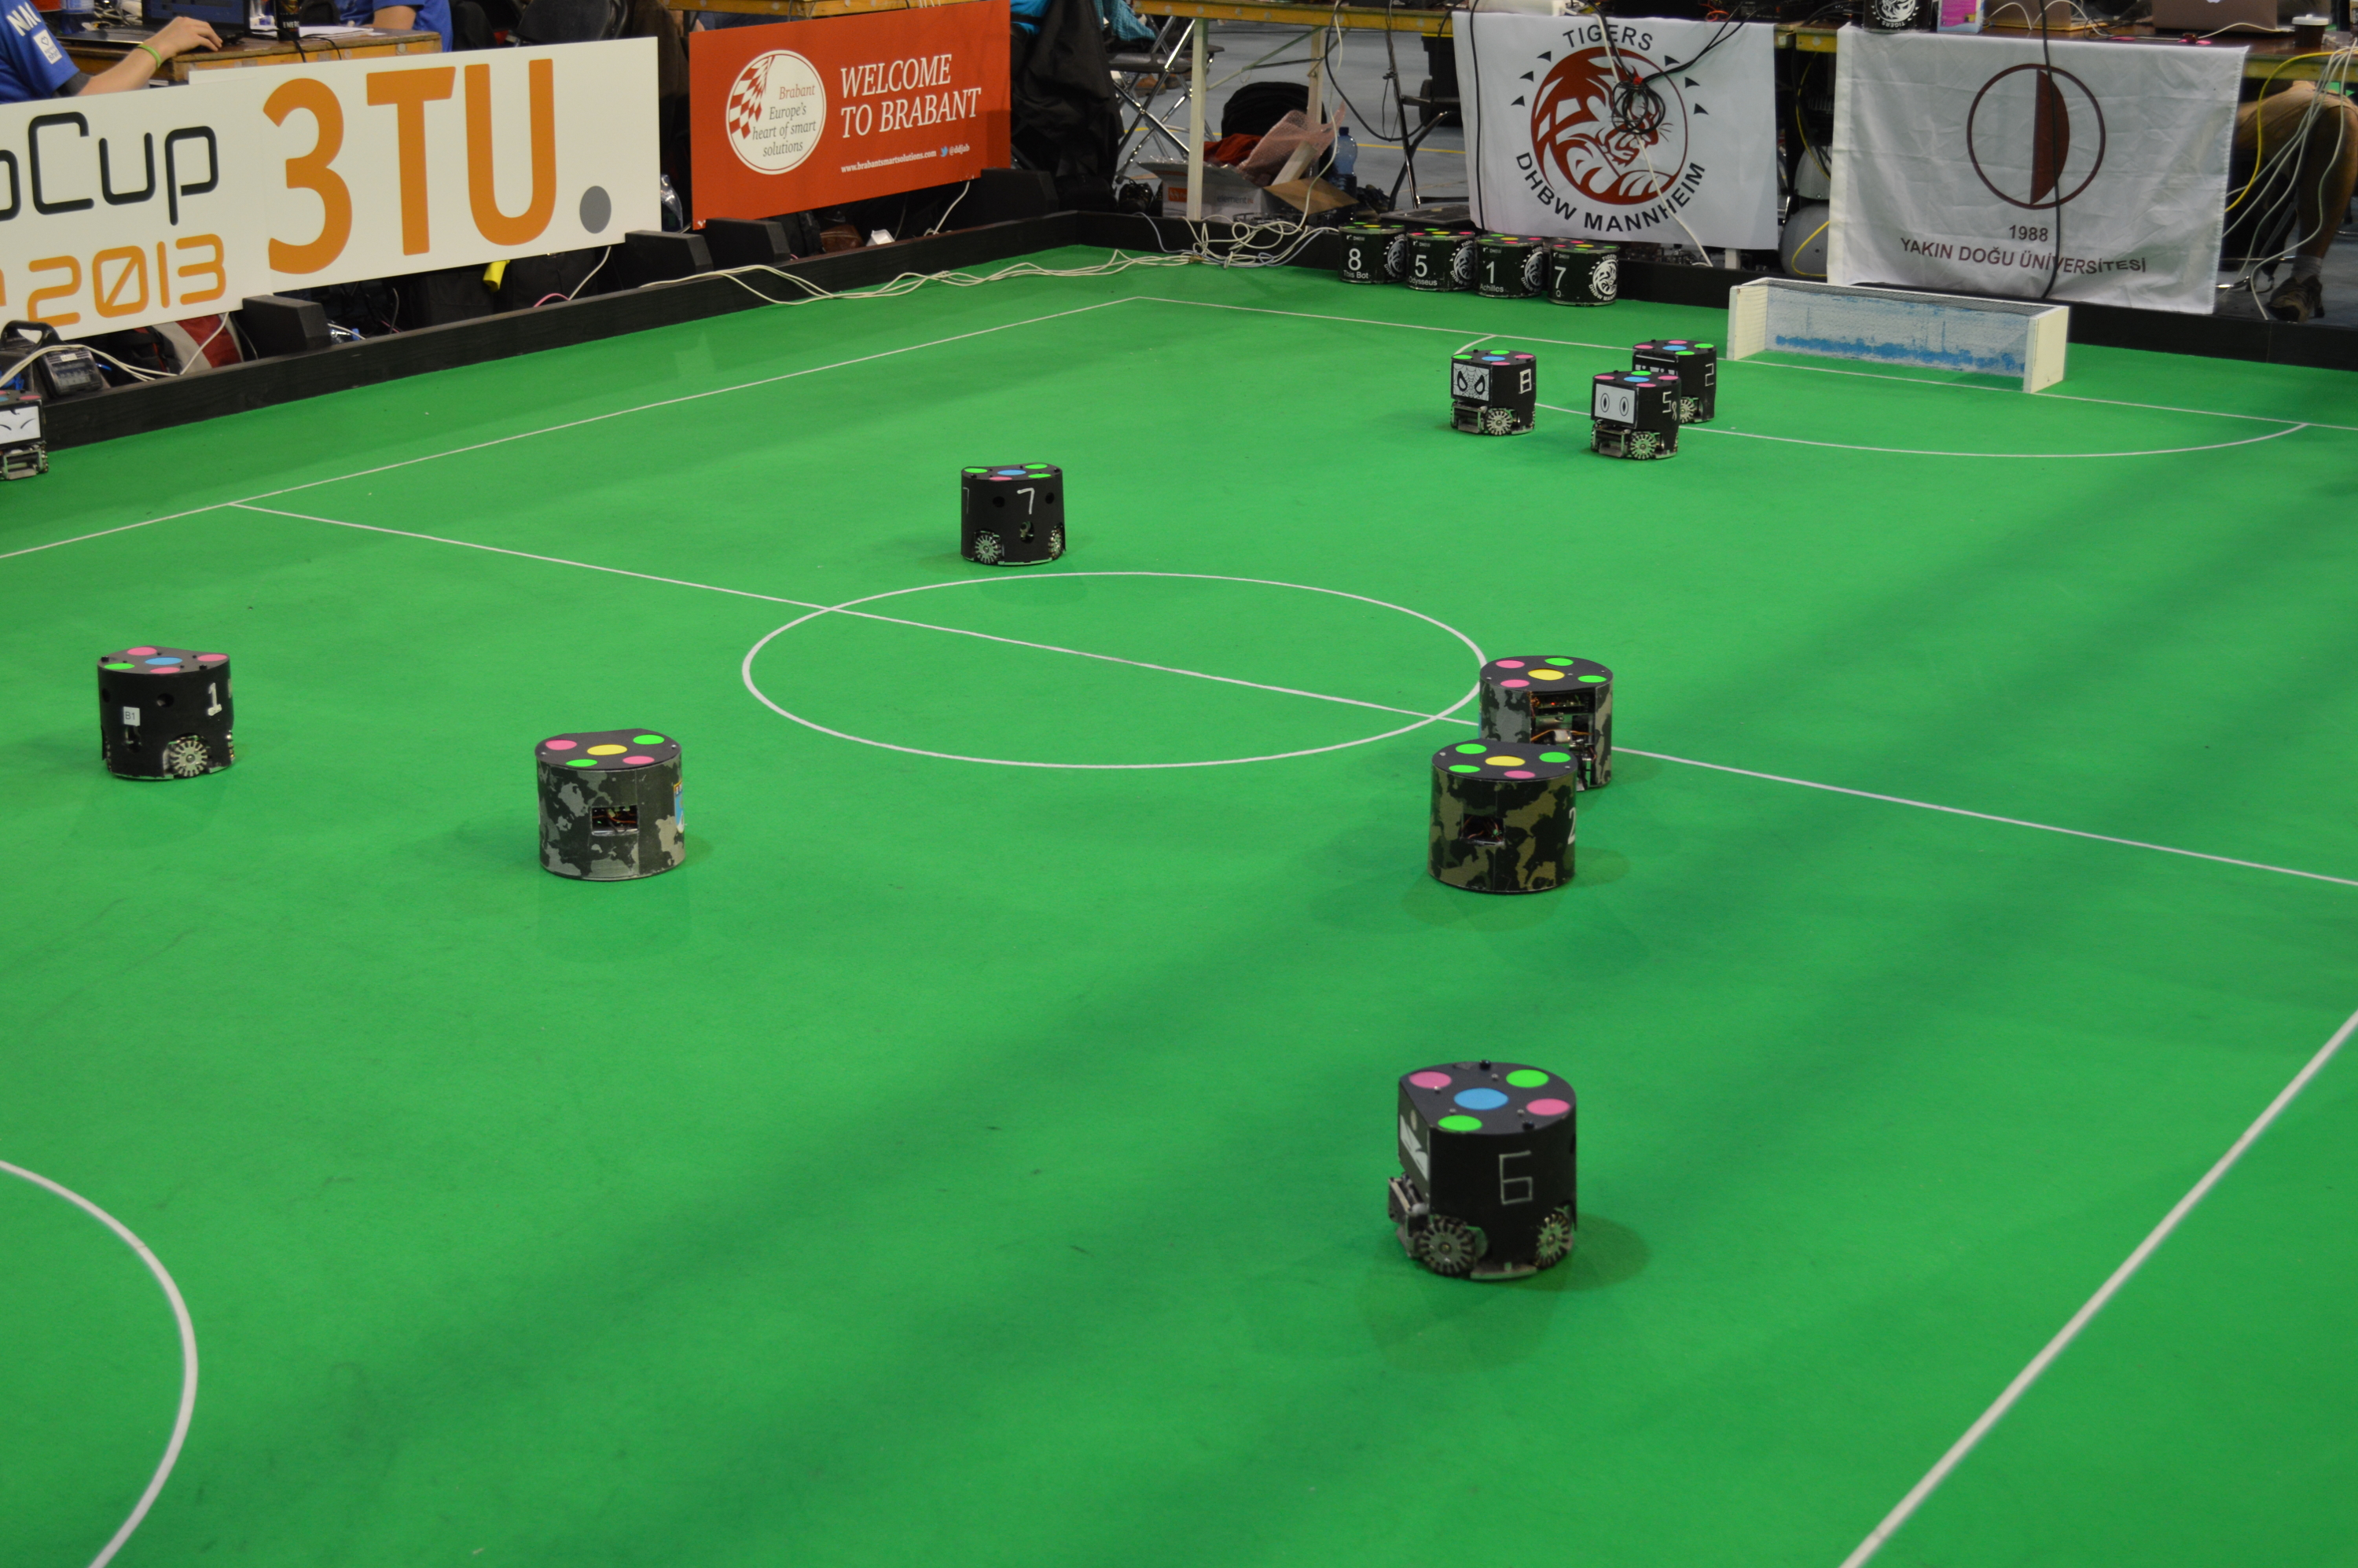
\includegraphics[width = \linewidth]{figuras/robocup2013}\label{robocup2013}
  \caption{Imagem da SSL \textit{RoboCup} 2013 em Eindhoven, na Holanda}
\end{figure}

A ideia de robôs jogando futebol foi mencionada pela primeira vez pelo professor
Alan Mackworth (\textit{University of British Columbia}, Canadá) em um artigo intitulado
\textit{"On Seeing Robots"}, apresentado no \textit{Vision Interface 92} e posteriormente publicado em
um livro chamado \textit{Computer Vision: System, Theory and Applications}. Independentemente,
um grupo de pesquisadores japoneses organizou um \textit{Workshop} no \textit{Ground Challange
in Artificial Inteligence}, em Outubro de 1992, Tóquio, discutindo e propondo problemas que
representavam grandes desafios. Esse \textit{Workshop} os levou a sérias discussões sobre
usar um jogo de futebol para promover ciência e tecnologia. Estudos foram feitos para
analisar a viabilidade dessa ideia. Os resultados desses estudos mostram que
a ideia era viável, desejável e englobava diversas aplicações práticas. Em 1993, um
grupo de pesquisadores, incluindo Minoru Asada, Yasuo Kuniyoshi e Hiroaki Kitano,
lançaram uma competição de robótica chamada de Robot \textit{J-League} (fazendo uma analogia à
\textit{J-League}, nome da Liga Japonesa de Futebol Profissional). Em um mês, vários
pesquisadores já se pronunciavam dizendo que a iniciativa deveria ser estendida ao
âmbito internacional. Surgia então, a \textit{Robot World Cup Initiative} (RoboCup).

RoboCup é uma competição destinada a desenvolver os estudos na área de robótica e
Inteligência Artificial (IA) por meio de um competição amigável. Além disso, ela tem
como objetivo, até 2050, desenvolver uma equipe de robôs humanoides totalmente
autônomos capazes de derrotar a equipe campeã mundial de futebol humano. A competição
possui várias modalidades. Neste trabalho, será analisada a \textit{Small Size Robot League} (SSL),
também conhecida como F180. De acordo com as regras da SSL, as equipes devem ser
compostas por 6 robôs, sendo um deles o goleiro, que deve ser
designado antes do início do jogo. Durante o jogo, nenhuma interferência humana é
permitida com o sistema de controle dos robôs. É fornecido aos times um sistema de
visão global e esses controlam seus robôs com máquinas próprias. O sistema de controle
dos robôs geralmente é externo e recebe os dados de um conjunto de duas câmeras
localizadas acima do campo. Esse sistema de controle processa os dados, determina qual comando deve ser executado por
cada robô e envia este comando através de ondas de rádio aos robôs. Embora seja
permitido que as equipes utilizem sistemas próprios de visão, a maioria das
equipes utiliza a visão centralizada. A figura~\ref{robocup2013} mostra uma
imagem da SSL Robocup 2013, da qual a RoboIME (Equipe de Futebol de Robôs do
Laboratório de Robótica do IME) participou.

\section{Motivação}

O futebol de robôs, problema padrão de investigação internacional, reúne grande parte
dos desafios presentes em problemas do mundo real a serem resolvidos em tempo real.
As soluções encontradas para o futebol de robôs podem ser estendidas, possibilitando
o uso da robótica em locais de difícil acesso para humanos, ambientes insalubres e
situações de risco de vida iminente.

Há diversas novas áreas de aplicação da robótica, tais como exploração espacial e submarina,
navegação em ambientes inóspitos e perigosos, serviço de assistência médica
e cirúrgica, além do setor de entretenimento. Essas áreas podem ser beneficiadas com o
desenvolvimento de sistemas
multi robôs. Nestes domínios de aplicação, sistemas de multi robôs deparam-se sempre
com tarefas muito difíceis de serem efetuadas por um único robô. Um time de robôs pode
prover redundância e contribuir cooperativamente para resolver o problema em questão.
Com efeito, eles podem resolver o problema de maneira mais confiável, mais rápida e
mais econômica, quando comparado com o desempenho de um único robô.

% TODO Incluir imagem do robô
%\begin{figure}
%  \includegraphics[width = \pagewidth]{}
%\end{figure}

Devido à grande complexidade do problema de interação com humanos, faz-se necessário
que os robôs sejam dotados de uma capacidade de aprendizado para facilitar a interação
desses com o mundo real. Isso é relevante tanto para aplicações industriais, quanto para
aplicações em resgates e militares. Isso diminui a necessidade de modelagem
exata dos ambientes em que os sistemas robóticos serão introduzidos e permite que
a adaptação a ambientes complexos seja realizada através da exposição destes sistemas
às possíveis situações de trabalho. Por meio da incorporação do sistema de
aprendizagem, situações não consideradas podem ser incorporadas ao algoritmo de
controle dos robôs dinamicamente. Isso permitiria que esses reagissem de maneira mais
eficiente em futuras situações semelhantes.

\section{Objetivo}

Este trabalho objetiva, através do processo de \textit{Mineração de Dados}, extrair
informação dos $logs$ (definido a seguir) de um jogo do futebol de robôs.
Isso tem o objetivo de permitir que agentes controláveis
possam reagir de maneira eficiente às ações dos agentes do time adversário, que não são controláveis.
A pesquisa se propõe a realizar esse aprendizado dos agentes adversários baseado em gravações
coletadas dos pacotes da \textit{SSL-Vision} e do \textit{Referee-Box} durante jogos, também conhecidas
como \textit{logs}, para posteriormente serem incorporados ao sistema de inteligência da
equipe de futebol de robôs do Laboratório de Robótica, denominada RoboIME.
% NOTE: acho que não é o caso disso:
%Se possível, deseja-se que essa modelagem/aprendizagem seja feita dinamicamente durante a partida da SSL.

\section{Justificativa}% TODO Maj Duarte colocou um certo nessa encestação

Um método concreto que possa prever o comportamento de agentes inteligentes de um jogo de
futebol de robôs permite com que seja possível prever o comportamento de um time adversário.
Com tal mecanismo é possível melhorar a Inteligência Artificial em uso pela RoboIME
para tomar decisões que levem a resultados melhores e, por consequência, ganhar mais partidas.
Outras equipes participantes da SSL já utilizam mecanismos de predição do adversário.
Portanto, é de grande importância desenvolver também tal mecanismo para acompanhar a evolução
das tecnologias envolvidas.

\section{Metodologia}

Para atingir os objetivos propostos, será seguida a seguinte metodologia:
Inicialmente o problema a ser investigado será definido formalmente,
utilizando definições e teorias apropriadas.

Posteriormente, a bibliografia é revisada e são evidenciados os métodos comumente
utilizados para a abordagem do problema mais geral de classificação, bem como são
analisados trabalhos aplicados especificamente à SSL.

A seguir, são analisadas as heurísticas levantadas durante a
revisão da bibliografia. Cada uma delas é descrita. Após descrição sumária
de cada heurística, são apresentados os respectivos exemplos de cada aplicação.

Então, são apresentadas abordagens envolvendo as heurísticas introduzidas
anteriormente. Cada abordagem relaciona, no mínimo, uma dessas heurísticas.
Ao final de cada seção, é apresentado uma metodologia a ser aplicada
na resolução do problema. Uma análise das características de cada abordagem
é feita ao final da descrição de cada abordagem.

A seguir, são descritos possíveis algoritmos para implementar essas abordagens. Também são
desenvolvidas métricas para avaliar os algoritmos desenvolvidos.

% NOTE: não é bem verdade isso:
%Para validar os estudos desenvolvidos, o projeto de um software
%que analise os dados dos \textit{logs} disponíveis no site da SSL é apresentado.

\section{Estrutura do Trabalho}

No capítulo~\ref{cap:def_problema}, o problema a ser resolvido é definido formalmente.

No capítulo~\ref{cap:rev_bibliografica}, a bibliografia é revisada.

No capítulo~\ref{cap:heuristicas}, são apresentados tutoriais relacionados às
heurísticas comumente utilizadas em problemas de classificação.

No capítulo~\ref{cap:anal_abordagens}, são descritas possíveis abordagens a serem
seguidas para resolução do problema.

No capítulo~\ref{cap:conclusao}, são apresentadas as principais conclusões atingidas.
